\documentclass[a4paper, 12pt, oneside]{article}
\usepackage[utf8]{inputenc}
\usepackage[margin=3cm, bindingoffset=1cm]{geometry}
\linespread{1.5}
\usepackage{float}
\usepackage{csquotes}
\usepackage{subfig}
\usepackage{graphicx}
\usepackage{indentfirst}
\usepackage{fancyhdr}
\usepackage{alphabeta}
\usepackage{algpseudocode}
\usepackage{algorithm}
\usepackage{hyperref}
\usepackage[T1]{fontenc}
\usepackage{listings}
\usepackage[htt]{hyphenat}
\usepackage{pgfplots}
\usepackage{wrapfig}

\usepackage[
    backend=biber,
    sorting=none
]{biblatex}
\addbibresource{bibliography.bib}


\setlength{\parindent}{1cm}

\pagestyle{fancy}
\fancyhf{}
\fancyhead[C]{\textbf{\leftmark}}
\fancyfoot[C]{\thepage}
\renewcommand{\headrulewidth}{1pt}
\renewcommand{\footrulewidth}{1pt}
\renewcommand{\contentsname}{Indice}
\usepackage{caption}
\captionsetup[figure]{labelformat=empty}

\usepackage[Conny]{fncychap}

  
\begin{document}
\begin{titlepage}
    \begin{center}
        \LARGE{\uppercase{Università degli Studi di Salerno}}\\
        \vspace{5mm}
    	\uppercase{\normalsize Dipartimento di Informatica }\\
    \end{center}
    \begin{figure}[H]
        \centering
        
\includegraphics[width=0.35\textwidth]{logo_unisa}
    \end{figure}
    
    \begin{center}
        \normalsize{\textbf{Corso di Laurea Magistrale in Informatica}}\\
    	\vspace{10mm}
    	\LARGE{\textbf{Securing \textsc{MAVLink} protocol: a Post Quantum cryptography-based approach}}\\
    	\vspace{3mm}
        \large{\uppercase{Anno Accademico 2022/2023}}
    \end{center}

    \vspace{50mm}
    \noindent
    \begin{minipage}[t]{0.4\textwidth}
    	\textsc{Relatore}\\Prof. \textbf{Arcangelo Castiglione}\\
        \small Università degli Studi di Salerno
    	\vspace{12mm}\\
    \end{minipage}
    \hfill
    \begin{minipage}[t]{0.4\textwidth}\raggedleft
    	\textsc{Candidato} \\\textbf{Hermann Senatore}\\\small Matricola: \textbf{0522501273}
    \end{minipage}
\end{titlepage}

\tableofcontents
\newpage

\begin{abstract}
    L'evoluzione tecnologica a cui si sta assistendo negli ultimi anni sta rivoluzionando pesantemente (tra le altre cose) il mondo dell'aviazione, merito anche (e soprattutto) dei cosiddetti \textbf{UAV} (unmanned aerial vehicle), che comunemente vengono definiti \textbf{droni}, impiegati sia in contesto "civile" che in contesto militare. 
    
    La potenziale delicatezza delle missioni che questi veicoli si trovano ad affrontare suggerisce dunque la necessità di definire dei requisiti di sicurezza che ne permettano un impiego più agevole. L'innovazione tecnologica porta però a nuove sfide anche nel campo della sicurezza. 
    
    In particolare, i recenti progressi nel campo del \textbf{quantum computing} apre nuove sfide nel contesto della crittografia, rendendo quindi necessario sviluppare nuove tecniche resistenti ad attacchi veicolati mediante computer quantistici. In questo lavoro viene presentato un \textbf{proof of concept} di un'architettura basata principalmente sul protocollo MAVLink che permetta una comunicazione sicura tra un drone e la sua \textbf{Ground Control Station} e, ad un livello più alto, la definizione della chiave di cifratura utilizzata mediante il \textbf{Key Encapsulation Mechanism} Kyber, selezionato dal \textbf{NIST} come lo standard per quanto riguarda gli algoritmi di incapsulamento \textbf{quantum resistant}.
\end{abstract}
\newpage

\section{Introduzione}

\subsection{Scopi e struttura della tesi}
Il presente lavoro si concentra, come tra l'altro già accennato in precedenza nell'abstract, sull'analisi del proof of concept di un'architettura basata sul protocollo MAVLink che permetta lo scambio di chiavi e la comunicazione cifrata tra un UAV e la sua centrale di comando a terra utilizzando il KEM quantum-resistant Kyber e l'algoritmo AES in modo tale da proteggere lo scambio di messaggi tra i due \textit{endpoint} della comunicazione.

In particolare:

\begin{itemize}
    \item Questo capitolo funge da introduzione al lavoro svolto durante l'attività di Tesi, ne illustra la struttura e ne chiarisce le motivazioni ed il contesto in cui è calato;
    \item il \textbf{Capitolo 2} fornisce una panoramica sulle principali piattaforme software considerate nel presente lavoro;
    \item il \textbf{Capitolo 3} fornisce una panoramica sul protocollo \textbf{MAVLink} e ne evidenzia alcune problematiche di sicurezza;
    \item il \textbf{Capitolo 4} fornisce un'introduzione all'impatto dell'avvento dei \textbf{Computer Quantistici} nel campo della crittografia e al concetto di \textbf{Post-Quantum Cryptography} (PQC). Si procederà quindi ad una panoramica dell'algoritmo \textbf{Kyber};
    \item il \textbf{Capitolo 5} illustra in dettaglio le \textbf{modifiche} effettuate alle piattaforme software considerate nel presente lavoro ed al protocollo MAVLink stesso;
    \item il \textbf{Capitolo 6} fornisce le \textbf{conclusioni} al presente lavoro e illustra alcuni possibili \textbf{sviluppi futuri}.
\end{itemize}

\newpage


\subsection{UAV, APR o Droni: nomenclatura}
Nell'ultimo decennio, l'importante evoluzione tecnologica nel contesto dell'aviazione ha permesso la progettazione e la concreta realizzazione di veicoli in grado di volare e compiere missioni anche \textbf{senza la presenza di un pilota umano} sempre più versatili, efficaci e precisi. Questa tipologia di veicoli viene definita, a seconda del contesto linguistico in cui ci si trova, \textbf{UAV} (\textit{unmanned aerial vehicle}), \textbf{APR} (\textit{aeromobile a pilotaggio remoto}) o, più comunemente, \textbf{Drone}. Tutti questi acronimi sono, quindi, equivalenti tra di loro. 

La presenza di un essere umano continua tuttavia ad essere fondamentale in quanto il pilotaggio di questi dispositivi viene effettuato mentre una struttura di controllo "a terra", che prende il nome di \textbf{Ground Control Station} (da qui in poi \textit{GCS}). Tipicamente, una GCS può essere rappresentata da un qualsiasi apparato in grado di comunicare in qualche modo con l'UAV, quindi anche un comune Personal Computer su cui viene posto in esecuzione un software specifico.

\subsection{Cenni storici}
Il concetto di aeromobile senza pilota in sé non è sorprendentemente prerogativa degli ultimi anni e delle conseguenze che l'avvento delle tecnologie informatiche si porta dietro. Risale infatti agli Anni '40 del XIX secolo il primo (rudimentale!) impiego di "dispositivi" volanti senza pilota in campo militare. 

Per fronteggiare i moti rivoluzionari, peraltro diffusi anche in tutta Europa nel 1848, nella città di Venezia (che avevano portato alla creazione della cosiddetta Repubblica di San Marco), l'esercito austriaco lanciò dei \textbf{palloni} a cui era stato fissato dell'\textbf{esplosivo} dalla nave "Vulcano". 

Questo primo esperimento portò a risultati "misti": alcuni di questi dispositivi riuscirono effettivamente a colpire la città, altri furono invece deviati dal vento.

Per tutto il XIX secolo, lo sviluppo di questo tipo di dispositivi rimase prerogativa militare, con gli americani e gli inglesi che si occuparono dello sviluppo dei primi aeromobili comandati tramite radiofrequenza. Questi ultimi, nel 1917, testarono con successo un velivolo chiamato \textbf{Aerial Target}, mentre gli americani misero a punto il cosiddetto \textbf{Kettering Bug} \cite{drones-history}.

Nessuno di questi due prototipi venne tuttavia impiegato nella \textbf{prima guerra mondiale}.

Come già accennato in precedenza, con il passare del tempo e con il sempre più spinto progresso tecnologico i droni e, più in generale i veicoli a guida remota, hanno trovato un fertile campo di applicazione anche nell'ambito \textbf{civile}. Ad esempio, nel 2022 è stato proposto uno studio in cui è stato utilizzato un insieme di veicoli senza pilota per monitorare il processo di realizzazione di un \textbf{ponte} \cite{rs14081858}.
Si è assistito, riassumendo, ad una "democratizzazione" dell'uso dei droni negli ambiti più disparati.

\subsection{Sviluppi recenti}
Proprio questa diffusione più capillare dell'uso di suddetti veicoli a guida remota ha portato ad una più grande attenzione nello sviluppo di tecnologie software specifiche a questo ambito. 

A partire dagli anni 10 del XXI secolo sono stati concepiti diversi progetti software \textbf{open source} che forniscono piattaforme integrate compatibili con diversi tipi di apparati sia lato UAV che lato GCS. 

Parimenti, è stato necessario definire uno \textit{standard} per quanto riguarda l'ambito dei protocolli di comunicazione tra il drone e la sua \textit{GCS}, che è rappresentato sicuramente dal protocollo \textbf{MAVLink} e dalle sue successive evoluzioni. 

Una panoramica più approfondita sul protocollo MAVLink verrà in ogni caso affrontata nelle prossime sezioni in cui verranno illustrate le piattaforme software utilizzate nell'ambito del presente lavoro.

\newpage

\section{Piattaforme software per UAV e GCS}
Il presente capitolo fornisce una panoramica delle principali tecnologie utilizzate in ambito \textbf{civile} ed \textbf{amatoriale} nel contesto dei velivoli a pilotaggio remoto. In particolare viene riservata particolare attenzione ai seguenti due progetti \textbf{open source}:

\begin{itemize}
    \item \textbf{ArduPilot}: una piattaforma integrata scritta in \textbf{C++} utilizzabile su diverse tipologie di veicoli non necessariamente adatti al volo;
    \item \textbf{QGroundControl}: una \textbf{Ground Control Station} open source scritta in C++, che utilizza il framework \textbf{Qt} e che permette una più stretta interazione con la piattaforma ArduPilot.
\end{itemize}

\begin{figure}[H]
    \centering
    
\includegraphics[width=0.8\textwidth]{images/ardupilot_logo.png}
    \caption{Il logo di ArduPilot}
\end{figure}
\begin{figure}[H]
    \centering
    
\includegraphics[width=0.8\textwidth]{images/QGC_RGB_Logo_Horizontal_Positive_PREFERRED.png}
    \caption{Il logo di QGroundControl}
\end{figure}

Viene quindi svolta una panoramica sul protocollo di comunicazione \textbf{MAVLink} che permette l'interazione tra queste due componenti.

\begin{figure}[H]
    \centering
    
\includegraphics[width=0.8\textwidth]{images/logo_mavlink_small.png}
    \caption{Il logo del protocollo MAVLink}
\end{figure}

\newpage

\subsection{ArduPilot}

ArduPilot, come accennato, è una suite software universale che permette il controllo di diversi veicoli \textbf{non necessariamente volanti} \cite{ardupilot} la cui nascita risale al 2007.  L'idea di una suite software quale ArduPilot è stata formalizzata presso la piattaforma \textbf{DIYDrones.com}, community dedicata agli UAV fondata da \textbf{Chris Anderson} e che si definisce quindi "The Birthplace of ArduPilot"\cite{diy-drones}.

Nel 2009 venne prodotta la prima \textbf{board} che utilizzava questa piattaforma e nel novembre dello stesso anno il codice sorgente del progetto venne reso pubblico (ed è attualmente disponibile su GitHub all'url \url{https://github.com/ArduPilot/ardupilot})\cite{ardupilot-history}.

Correntemente, il progetto permette l'utilizzo su diverse tipologie di dispositivi, mediante delle versioni del firmware leggermente diverse tra di loro. In particolare, ArduPilot supporta dispositivi del tipo:

\begin{itemize}
    \item \textbf{Copter}: probabilmente quello più diffuso tra tutti e che tipicamente è composto da una board a cui sono associate diverse \textbf{eliche}. Il progetto di riferimento si chiama \textbf{ArduCopter}\cite{arducopter};
    \item \textbf{Plane}: un tipo di dispositivo ad \textbf{ala fissa}, tipicamente un \textbf{aereo radiocomandato}. Il progetto di riferimento si chiama \textbf{ArduPlane}\cite{arduplane};
    \item \textbf{Rover}: un tipo di dispositivo che non può spiccare il volo ma dotato di ruote e che di conseguenza viene utilizzato per missioni "a terra". Il progetto di riferimento si chiama semplicemente \textbf{Rover}\cite{rover};
    \item \textbf{Sub}: un tipo di dispositivo subacqueo, appartenente alla categoria degli \textbf{Autonomous Underwater Vehicles} (\textit{AUV}). Il progetto di riferimento si chiama \textbf{ArduSub}\cite{ardusub};
\end{itemize}

\begin{figure}[H]
    \centering
    \subfloat[\centering Copter]{{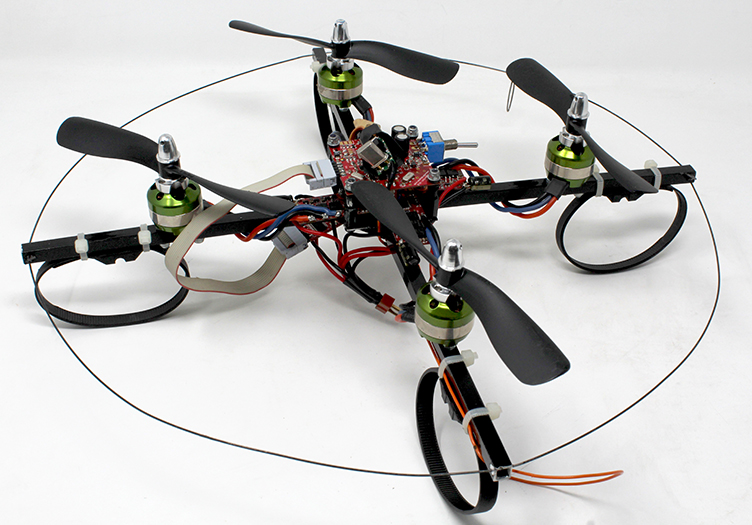
\includegraphics[width=0.4\textwidth]{images/copter.jpg} }}
    \qquad
    \subfloat[\centering Plane]{{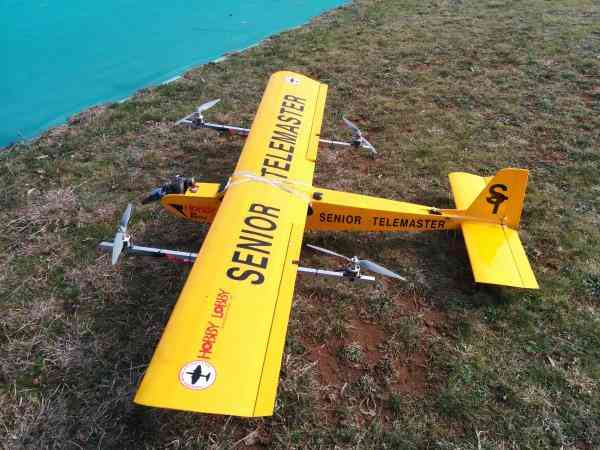
\includegraphics[width=0.4\textwidth]{images/plane.jpg} }}
\end{figure}
\begin{figure}[H]
    \centering
    \subfloat[\centering Rover]{{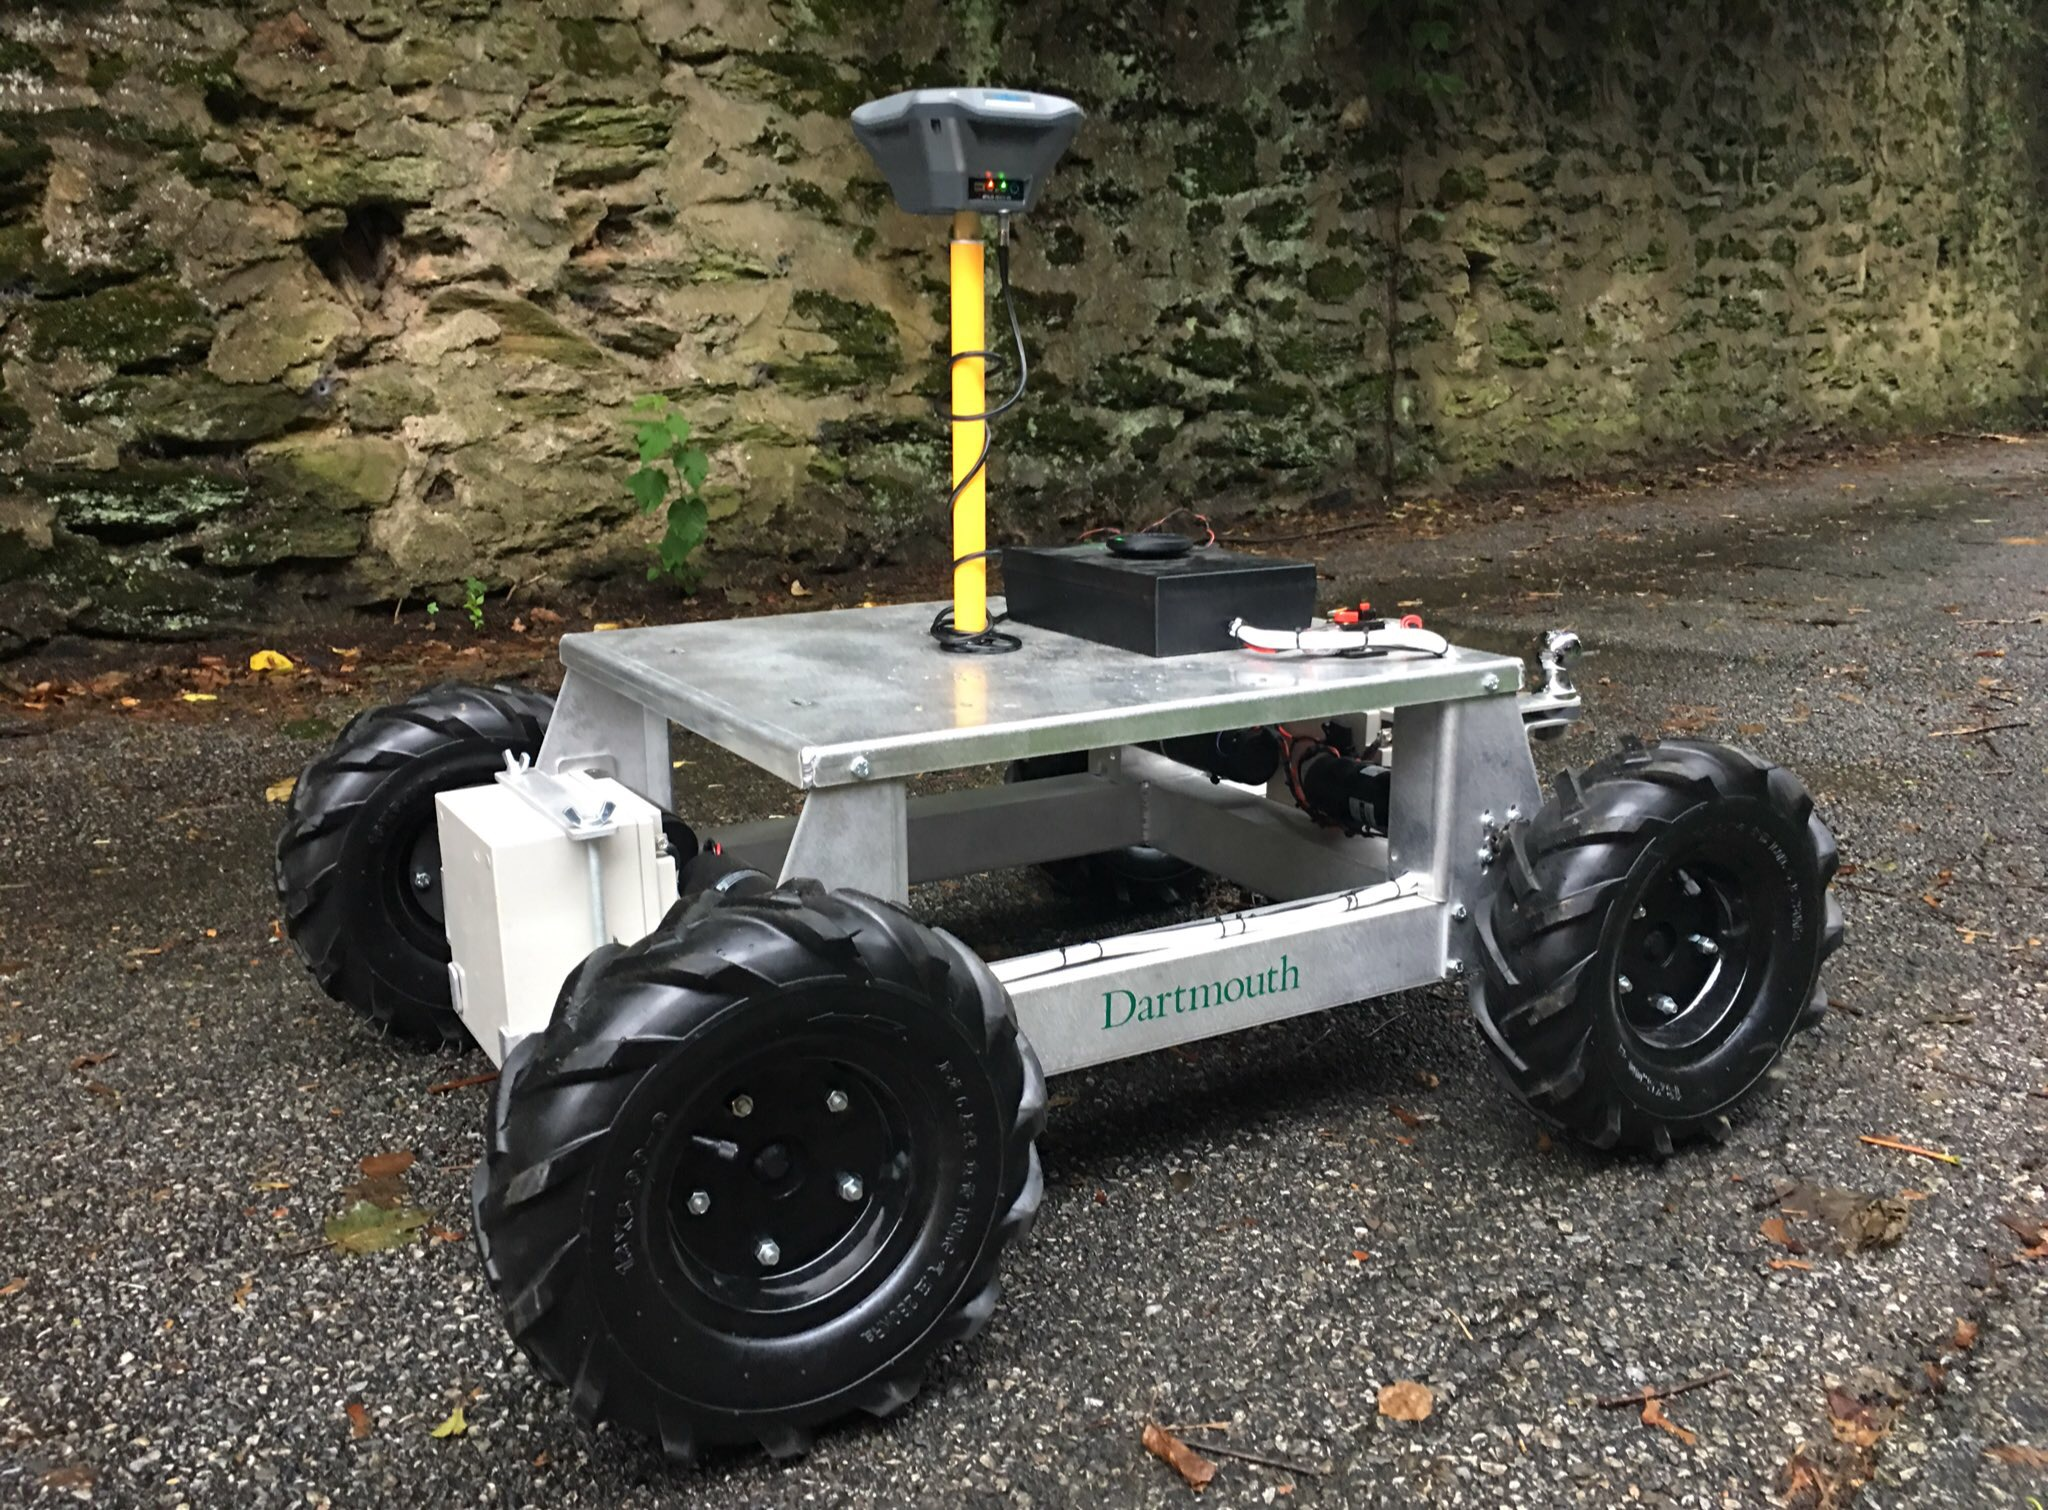
\includegraphics[width=0.4\textwidth]{images/rover.jpeg} }}
    \qquad
    \subfloat[\centering Sub]{{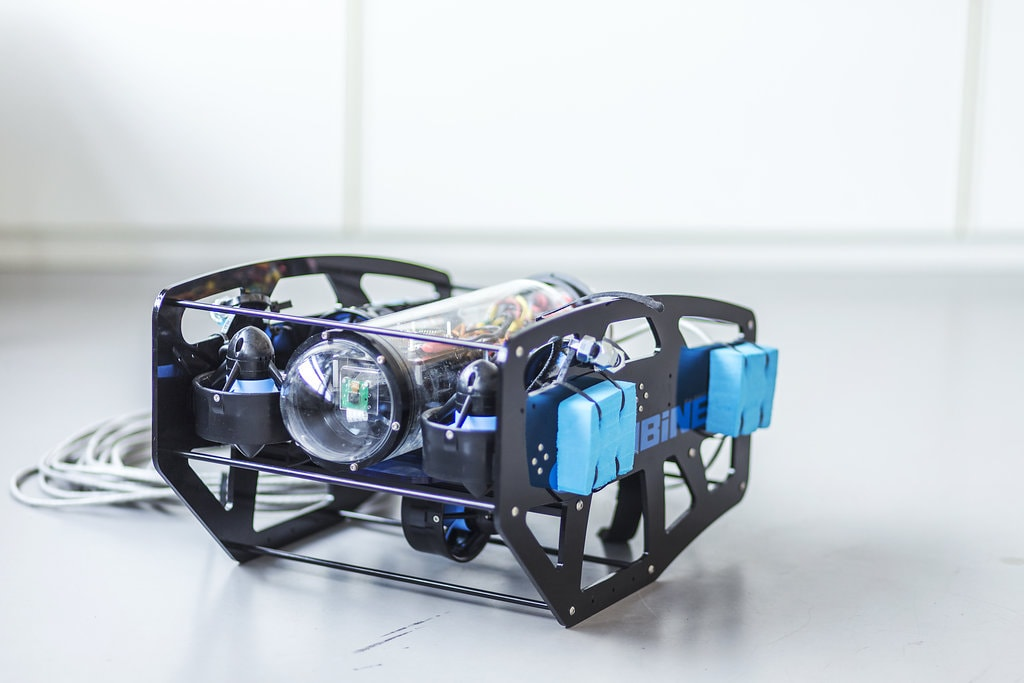
\includegraphics[width=0.4\textwidth]{images/sub.jpeg} }}
\end{figure}

Il progetto fornisce anche del codice specifico per apparati "complementari" ai dispositivi qui sopra descritti. In particolare:

\begin{itemize}
    \item \textbf{AntennaTracker}: che permette di governare apparati che si occupano di ricevere il segnale proveniente dai dispositivi controllati da remoto\cite{antennatracker};
    \item \textbf{Blimp}: un particolare tipo di "pallone" aerostatico dotato di motore\cite{blimp}.
\end{itemize}

\begin{figure}[H]
    \centering
    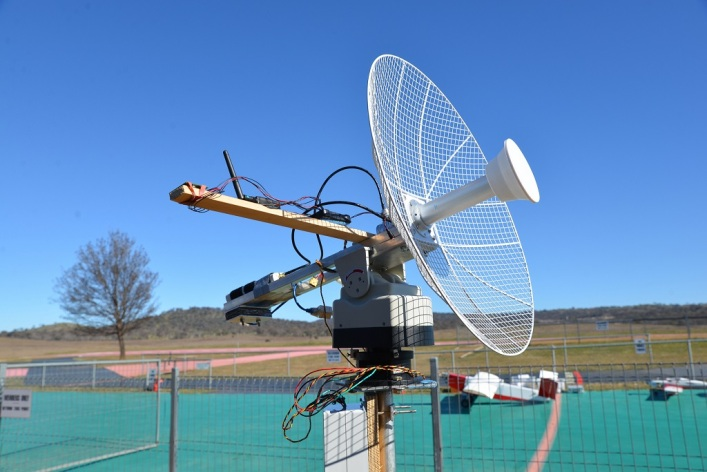
\includegraphics[width=0.8\textwidth]{images/antenna.jpg}
    \caption{AntennaTracker}
\end{figure}
\begin{figure}[H]
    \centering
    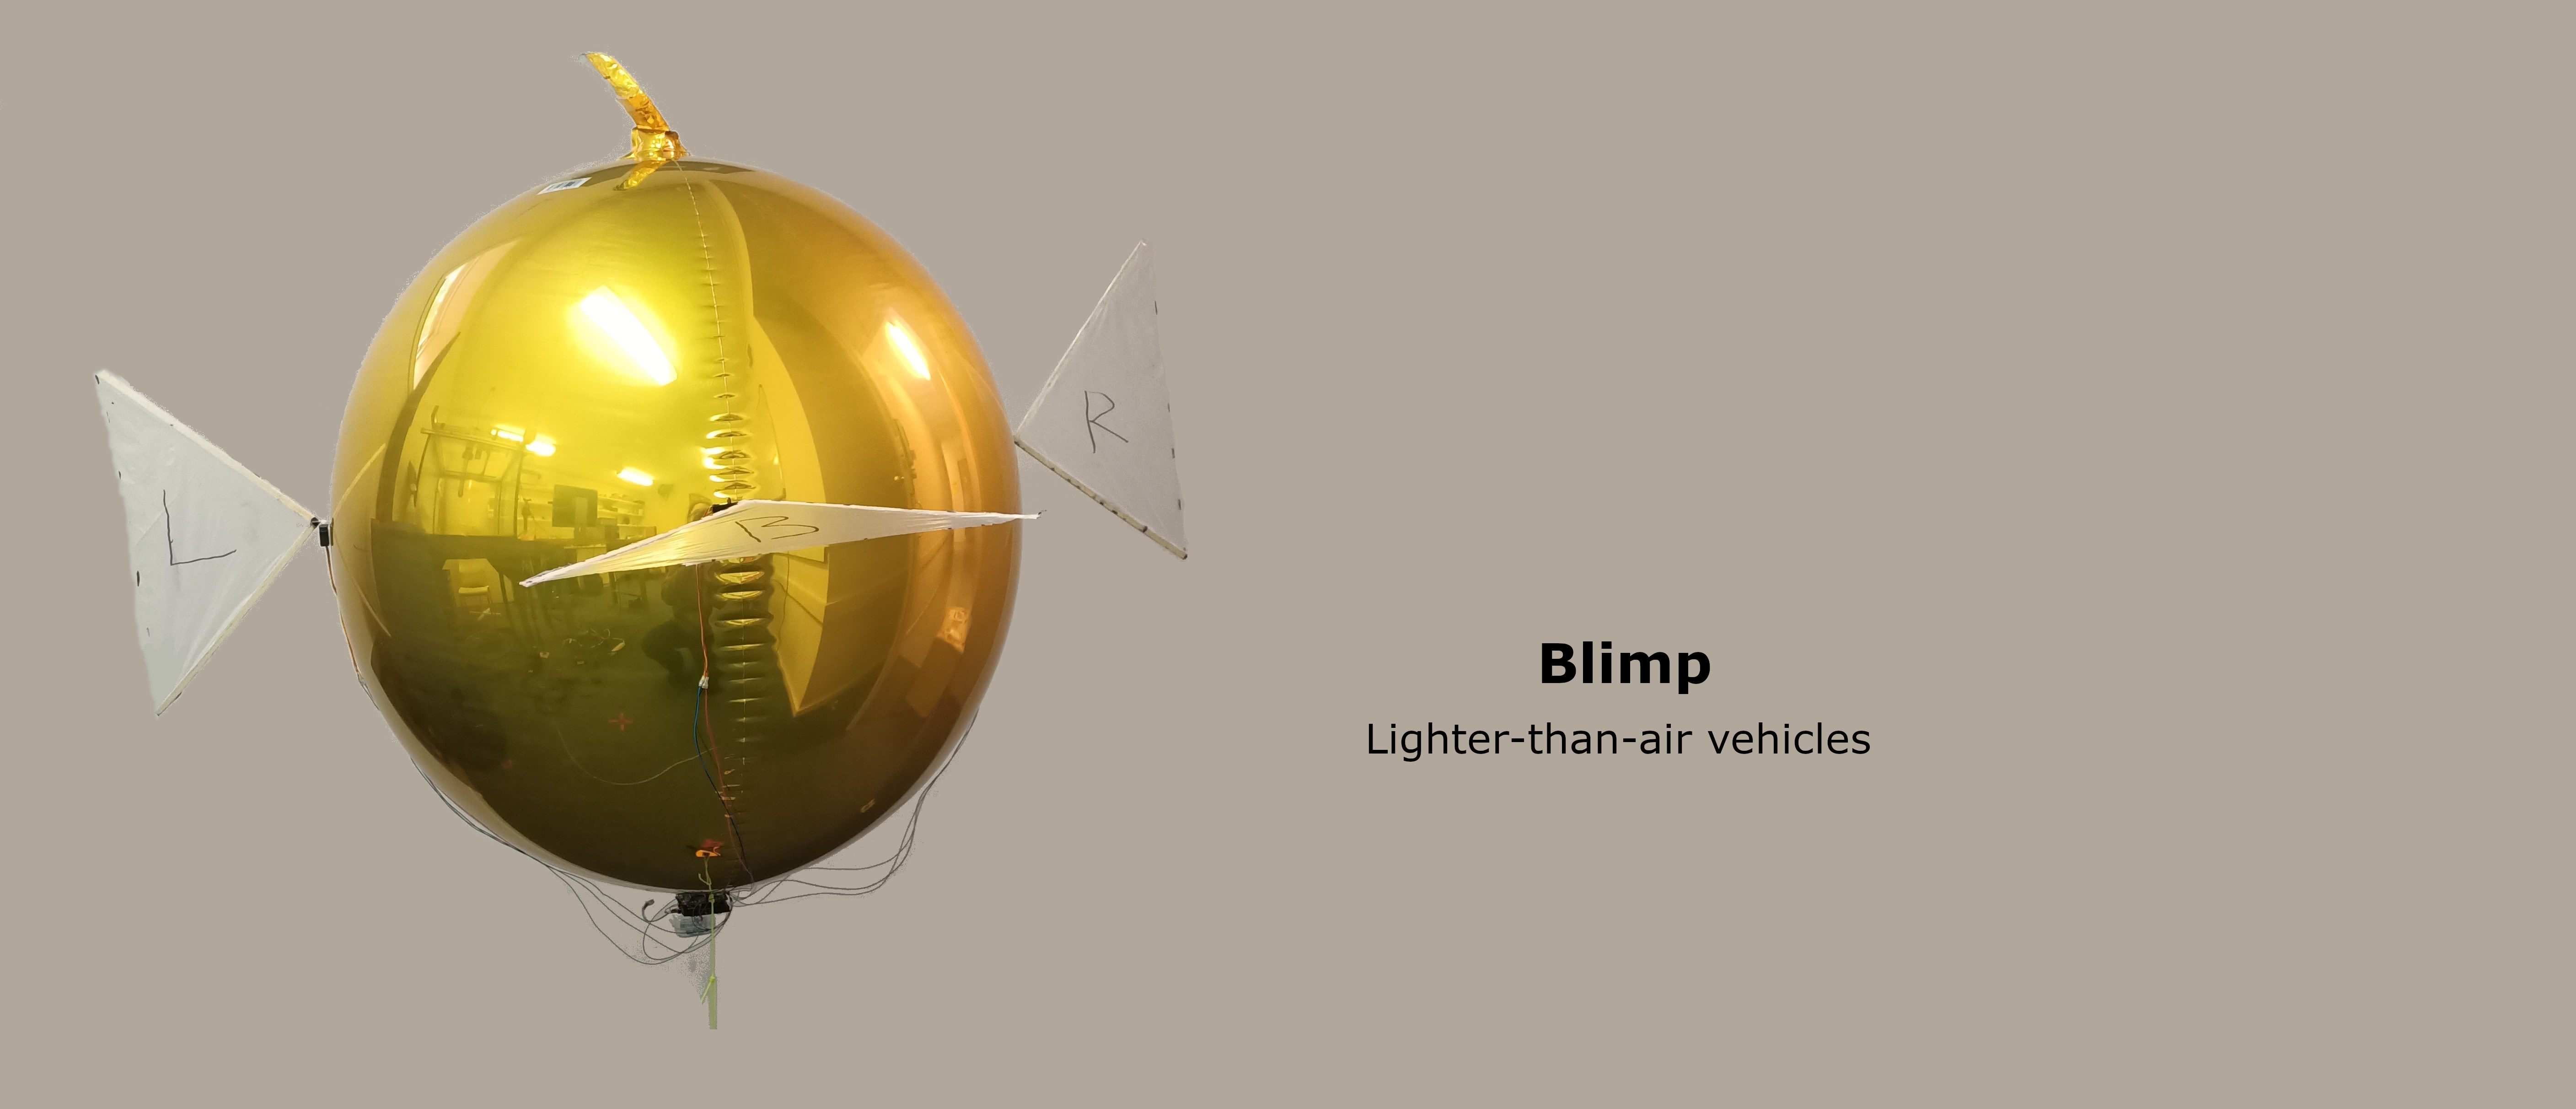
\includegraphics[width=0.8\textwidth]{images/blimp.png}
    \caption{Blimp}
\end{figure}

\subsubsection{SITL - Software in the Loop}
Il progetto ArduPilot mette inoltre a disposizione anche un \textbf{emulatore} che permette il testing di tutte queste varianti della piattaforma \textbf{senza possedere l'hardware adatto} \cite{sitl} e quindi procedere al \textbf{flashing} del firmware. 

Tale emulatore prende il nome di \textbf{SITL} (\textit{Software In The Loop}) e risulta quindi molto utile quando è necessario svolgere attività di testing preliminari per valutare il comportamento del firmware in use case differenti. 

Tra l'altro, proprio l'utilizzo di SITL ha permesso la realizzazione di questo lavoro in totale autonomia da hardware specifico. 

Maggiori informazioni su SITL e sul suo utilizzo saranno proposte in una successiva sottosezione dove verranno presentati ulteriori dettagli sull'architettura software del progetto ArduPilot.

\subsubsection{ArduPilot: architettura software}
Come menzionato in precedenza, il progetto ArduPilot utilizza il linguaggio di programmazione \textbf{C++}, che è uno di quelli più utilizzati per la programmazione di sistemi embedded in generale poiché \textbf{gira direttamente sull'hardware} senza bisogno di macchine virtuali di sorta (al contrario di Java o di linguaggi interpretati), permettendo di ottenere prestazioni migliori in un contesto in cui proprio le prestazioni rappresentano un requisito fondamentale.

Dal punto di vista della configurazione del progetto, la scelta degli sviluppatori di ArduPilot è ricaduta sul framework \textbf{waf}. Tale framework, scritto in Python, offre un ambiente di build modulare e per quanto possibile agnostico rispetto ai linguaggi di programmazione utilizzati nel progetto col quale lo si vuole usare.

In breve, la documentazione di waf \cite{waf} suggerisce che:

\begin{itemize}
    \item Per utilizzare il framework è necessaria unicamente un'installazione di \textbf{Python};
    \item Waf non definisce un nuovo "linguaggio" (come avviene nel meccanismo dei \textbf{Makefile}) ma si compone di moduli scritti in Python, che permette quindi una maggiore riusabilità delle componenti;
    \item I "target" sono definiti come oggetti python dichiarati in maniera separata dai comandi (definiti invece come funzioni in un file chiamato \texttt{wscript}).
\end{itemize}

\subsubsection{Compilare ArduPilot}

Il progetto GitHub della piattaforma ArduPilot contiene il codice sorgente specifico di tutte le tipologie di veicolo, organizzato in directory separate\cite{ardupilot-github}. In particolare:

\begin{itemize}
    \item \texttt{ArduCopter/} contiene il codice sorgente specifico per i veicoli di tipo \textbf{Copter};
    \item \texttt{ArduPlane/} contiene il codice sorgente specifico per i veicoli di tipo \textbf{Plane};
    \item \texttt{ArduSub/} contiene il codice sorgente specifico per i veicoli di tipo \textbf{Sub};
    \item \texttt{Rover/} contiene il codice sorgente specifico per i veicoli di tipo \textbf{Rover};
    \item \texttt{AntennaTracker/} contiene il codice sorgente specifico per i dispositivi che comandano \textbf{antenne di invio/ricezione};
    \item \texttt{Blimp/} contiene il codice sorgente specifico per i veicoli di tipo \textbf{Blimp}, come descritti in precedenza;
\end{itemize}

Inoltre, mediante il comando \texttt{configure} ed il parametro \texttt{-{}-board=} è possibile personalizzare ulteriormente la compilazione del firmware adattandolo ad un \textit{tipo di board} specifico o istruendo il sistema a prepararsi ad essere utilizzato mediante \textbf{SITL}\cite{how-to-build-ardupilot}. Quest'ultimo scenario è quello utilizzato nel presente lavoro e si ottiene eseguendo il comando:

\begin{center}
    \texttt{./waf configure -{}-board=sitl}
\end{center}

e, per generare il firmware specifico per un determinato tipo di veicolo (in questo caso quello di elezione è \textbf{Copter}), è necessario eseguire il seguente comando:

\begin{center}
    \texttt{./waf copter}
\end{center}

Per avviare l'emulatore \textbf{SITL} configurato in precedenza è necessario recarsi nella directory del veicolo per cui si è scelto di compilare il firmware (specificato nel comando precedente) (in questo caso, \texttt{ArduCopter/})

\begin{center}
    \texttt{cd ArduCopter/}
\end{center}

e finalmente eseguire l'emulatore mediante il comando

\begin{center}
    \texttt{sim\_vehicle.py}
\end{center}

Nota: il file appena descritto è presente nel percorso \texttt{/Tools/autotest/} ma non è necessario specificare il suo path assoluto perché durante l'installazione dei prerequisiti di ArduPilot, quest'ultimo viene aggiunto in maniera system-wide alla variabile d'ambiente \texttt{PATH}.

A questo punto, il veicolo "virtuale" è pronto ad accettare connessioni da una GCS. In particolare, viene aperta la porta \textbf{5760} sull'interfaccia di \textbf{loopback} locale.

È anche possibile modificare il numero di porta utilizzato e l'interfaccia su cui mettersi in ascolto.

\begin{figure}[H]
    \centering
    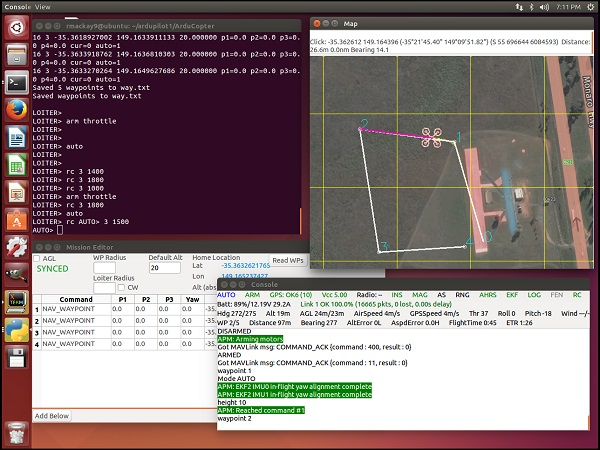
\includegraphics[width=0.8\textwidth]{images/sitl.jpg}
    \caption{SITL in esecuzione}
\end{figure}



\subsubsection{ArduPilot: integrazione con il protocollo MAVLink}
Il progetto ArduPilot usa il protocollo MAVLink per comunicare con le Ground Control Stations. Il codice sorgente che implementa le primitive e le funzioni di supporto per la comunicazione non è però già disponibile all'atto della clonazione del progetto da GitHub. Al contrario, è stato configurato il tool \texttt{mavgen} come \textit{submodule} all'interno della repository. Tale tool, richiamato dal sistema di building \texttt{waf} all'atto della compilazione del codice per un determinato veicolo, permette di generare \textit{dinamicamente} tutto il codice di basso livello necessario per le operazioni di comunicazione verso l'esterno\cite{mavgen}. Più nello specifico, viene generata una libreria \textit{headers-only} in linguaggio \textbf{C}, che tuttavia risulta perfettamente interoperabile con il resto del software scritto invece, come già menzionato, in C++. Maggiori dettagli su questo tool saranno forniti durante la panoramica che verrà svolta riguardo il protocollo MAVLink.

\newpage

\subsection{QGroundControl}

\subsubsection{Panoramica sulle principali GCS disponibili}

Come menzionato in precedenza, un UAV per essere totalmente operativo ha bisogno di una componente \textbf{"a terra"} che lo governi: questa componente prende appunto il nome di \textbf{Ground Control Station} (GCS) e si occupa di gestire la connessione con l'UAV mediante il protocollo più adatto e di controllarlo mediante messaggi tipicamente aderenti alle specifiche \textbf{MAVLink} (maggiori informazioni sono fornite nella sottosezione dedicata). È quindi pacifico affermare che il software in questione risulti essere nella maggior parte dei casi \textbf{molto complesso} dal punto di vista dei requisiti a cui deve rispondere e da quello dell'architettura software.

Attualmente, sono disponibili pubblicamente diverse Ground Control Station più o meno sofisticate. Tra queste si annoverano:

\begin{itemize}
    \item \textbf{MAVProxy} \cite{mavproxy}: una (non necessariamente) command-line-based GCS che possiede tutti gli strumenti necessari a comandare un UAV risultando al contempo utilizzabile su sistemi con a disposizione relativamente poche risorse. Di default, è quella che si avvia al momento dell'esecuzione di \textbf{SITL} a meno che non venga passato il parametro \texttt{-{}-no-mavproxy} allo script \texttt{sim\_vehicle.py} (come accennato in precedenza);
    \item \textbf{Mission Planner} \cite{mission-planner}, sviluppato da \textbf{Michael Orbone} e che permette di gestire diversi aspetti di una missione di un UAV: dalla configurazione dei waypoints (in termini di coordinate GPS) ai comandi da far eseguire all'UAV durante lo svolgimento della missione;
    \item \textbf{APM Planner 2}: sostanzialmente \textbf{un'evoluzione} dello strumento Mission Planner, creato dal team di sviluppo di \textbf{ArduPilot} e che permette di gestire sia dispositivi basati su ArduPilot stesso che basati sulla piattaforma \textbf{PX4};
    \item \textbf{QGroundControl} \cite{qgroundcontrol}: probabilmente la GCS più funzionale tra quelle appena descritte. È stata sviluppata dal team che si occupa del protocollo \textbf{MAVLink} e che permette di interfacciarsi con qualsiasi dispositivo che supporti i messaggi MAVLink. Tale piattaforma è stata utilizzata per realizzare parte del lavoro di tesi qui presentato. 
\end{itemize}

\subsubsection{Architettura software di QGroundControl}

Come accennato, QGroundControl è un software molto complesso e che fornisce una moltitudine di funzionalità, che vanno dalla pianificazione delle missioni al monitoraggio dei messaggi MAVLink tramite un \textbf{inspector} \textit{ad-hoc}, per citarne alcune.

Il progetto è stato sviluppato dall'organizzazione che si occupa di MAVLink e, più in generale, del \textbf{MAV-SDK}: la \textbf{DroneCode Foundation}, che ha come mission quella di "creare uno standard nell'industria dei droni mediante progetti open-source"\cite{dronecode}. 

È scritto interamente in \textbf{C++}, eccetto per lo stack di comunicazione MAVLink in uso, mediante l'ausilio del framework \textbf{Qt} ed il suo codice sorgente è disponibile su GitHub \cite{qgc-github}.

Al contrario delle altre GCS, QGroundControl \textbf{supporta anche la compilazione per la piattaforma Android}\cite{qgc-github-android}, il che di conseguenza permette l'utilizzo del software su dispositivi portatili e rendendo il progetto completamente \textbf{cross-platform}.

In ogni caso, il \textit{core} della piattaforma è presente all'interno della directory \texttt{src/} nella root della repo GitHub. Qui sono presenti tutti i moduli che permettono, tra le altre cose, la gestione dei veicoli connessi alla GCS (classe \texttt{Vehicle} coaudivata da un'istanza di \texttt{LinkManager}) e dei messaggi di cui è stato svolto il \textit{parsing} dalla libreria MAVLink (classe \texttt{MAVLinkProtocol}: presente nella sottodirectory \texttt{comm/}).

La comunicazione con l'UAV connesso avviene mediante \textbf{datagrammi UDP} gestiti da un \texttt{LinkManager} che contengono messaggi MAVLink costruiti utilizzando le funzioni della libreria C di questo progetto.

Al contrario di quanto avviene nel contesto di ArduPilot, con QGroundControl suddetta libreria \textbf{non viene generata} al momento della compilazione ma viene fatto uso dell'\textbf{implementazione di riferimento in C} \cite{mavlink-c-implementation} messa a disposizione pubblicamente da DroneCode su GitHub ed inclusa nella repo di QGroundControl utilizzando (ancora una volta) il meccanismo dei \textit{submodules}.

Il "dialetto" utilizzato di default da QGroundControl per la libreria MAVLink è (a partire dal 24 agosto 2023)\cite{qgc-all-commit} \texttt{all}, ma tale aspetto può essere variato in uno dei \textbf{file di configurazione del progetto}: \texttt{QGCExternalLibs.pri}.

Per quanto riguarda questo lavoro, invece, viene ancora utilizzato il "dialetto" \texttt{ArduPilotMega} poiché tale cambiamento non era stato proposto ed approvato. \footnote{Cambiamenti così importanti sono particolarmente frequenti in progetti open source del genere, ndr}

\subsubsection{Ottenere QGroundControl}
La natura open source e cross platform di tale progetto permette a chi è interessato di ottenerne una copia sostanzialmente in due modi:

\begin{enumerate}
    \item Utilizzando una \textbf{release} periodica precompilata;
    \item Compilando (ed eventualmente modificando!) il codice sorgente, approccio utilizzato tra l'altro nel presente lavoro.
\end{enumerate}

Per quanto riguarda la (1.), pacchetti precompilati sono disponibili nella sezione "release" di GitHub, dove sono presenti di solito:

\begin{itemize}
    \item Un file \texttt{.exe} che permette l'installazione su Microsoft Windows;
    \item Un'immagine disco \texttt{.dmg} montabile ed installabile su macOS;
    \item Un'\textit{AppImage} compatibile la maggior parte delle distro GNU/Linux;
    \item Un file apk installabile su Android.
\end{itemize}

Per quanto riguarda la (2.), sono naturalmente necessari particolari accorgimenti, oltre ad una piattaforma che permetta di compilare agevolmente un progetto di grandi dimensioni.\footnote{Gli step riportati qui di seguito si riferiscono al sistema operativo \textbf{Ubuntu 20.04 LTS}, lo stesso utilizzato per il lavoro presentato.}

In particolare:

\begin{enumerate}
    \item È necessario installare il framework \textbf{Qt}, mediante l'online installer oppure tramite tool di terze parti \cite{aqtinstall}. La versione di Qt necessaria attualmente è, secondo quanto indicato \cite{build-qgc}, la 5.15.2;
    \item Tramite il gestore pacchetti \texttt{apt} è necessario installare i seguenti pacchetti:
        \begin{itemize}
            \item \texttt{speech-dispatcher};
            \item \texttt{libudev-dev};
            \item \texttt{libsdl2-dev};
            \item \texttt{patchelf};
            \item \texttt{build-essential};
            \item \texttt{curl} (che probabilmente è già installato di default).
        \end{itemize}
\end{enumerate}

Successivamente è necessario preparare l'ambiente di build mediante i seguenti comandi nella \textit{root} della repository:

\begin{center}
    \texttt{mkdir build/ \&\& cd build/} \\
    \texttt{qmake ../}
\end{center}

L'invocazione di \texttt{qmake} permette a Qt di inizializzare i \textbf{Makefile} ed di caricare le \textbf{variabili d'ambiente} contenute nei \textbf{file di configurazione} (come ad esempio il dialetto di MAVLink da utilizzare, già accennato in precedenza).

È ora finalmente possibile invocare \texttt{make} per iniziare la procedura di compilazione vera e propria:

\begin{center}
    \texttt{make -j\$(nproc -{}-all)}
\end{center}

Il comando \texttt{nproc -{}-all} permette di determinare il numero di core logici che la CPU della macchina su cui si sta svolgendo la compilazione ha a disposizione. Ciò permette una compilazione veloce quanto più possibile.

Una volta terminata la compilazione del software, l'eseguibile prodotto sarà posizionato all'interno della cartella \texttt{build/staging} e si chiama semplicemente \texttt{QGroundContol}. Suddetto file ha già assegnati i permessi di esecuzione ed è possibile eseguirlo mediante il seguente comando:

\begin{center}
    \texttt{staging/QGroundControl}
\end{center}

\begin{figure}[H]
    \centering
    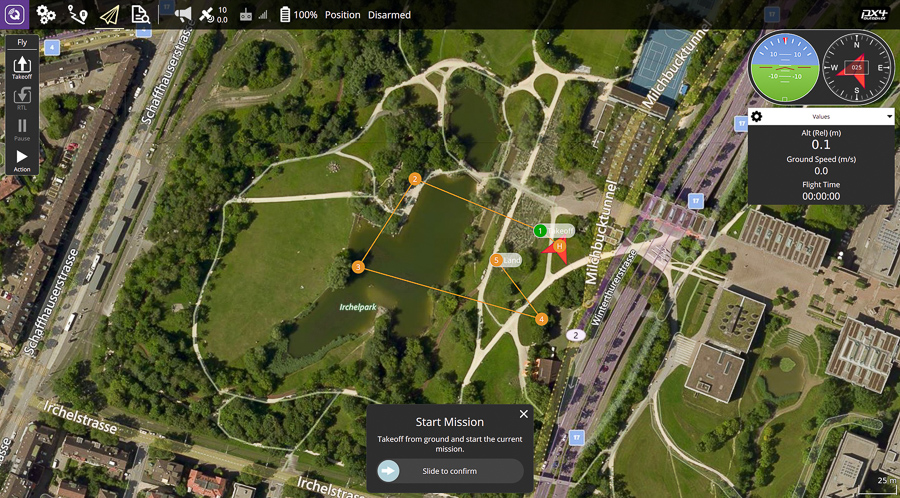
\includegraphics[width=0.8\textwidth]{images/QGroundCotrol-Interface.jpg}
    \caption{L'interfaccia di QGroundContol una volta aperto}
\end{figure}

\begin{figure}[H]
    \centering
    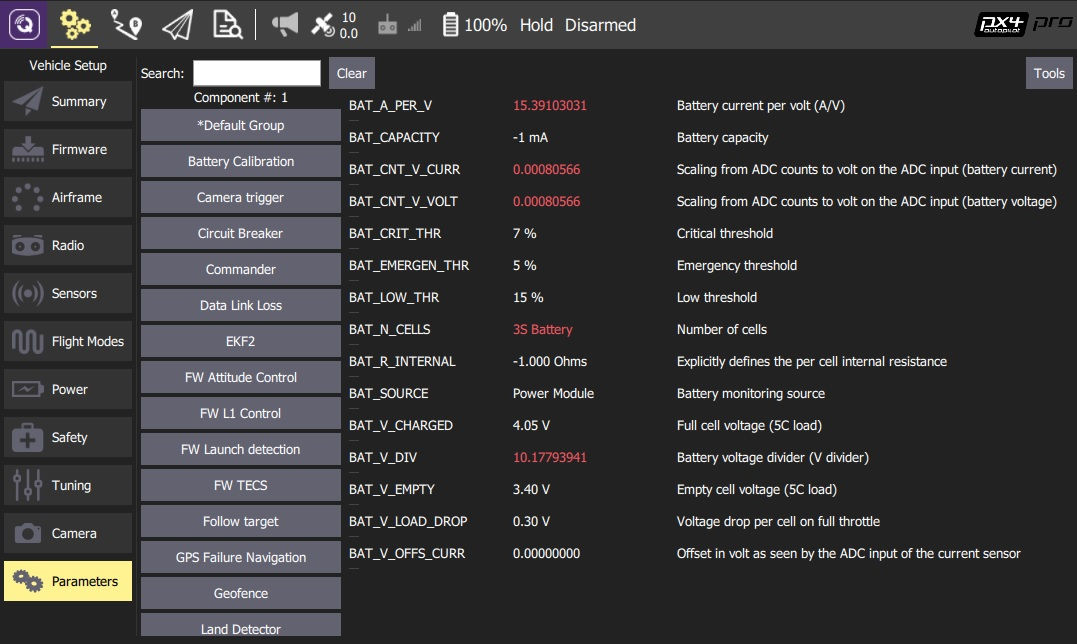
\includegraphics[width=0.8\textwidth]{images/QGroundControl-settings.jpg}
    \caption{Le impostazioni di QGroundContol}
\end{figure}

\section{Il protocollo MAVLink}

Come accennato in fase di introduzione a questo lavoro, il \textbf{protocollo MAVLink} è il vero e proprio "collante" tra le due parti della comunicazione, ovvero l'UAV e la GCS a terra. In questa sezione viene presentata la filosofia, le specifiche e l'architettura del protocollo MAVLink e se ne illustra l'evoluzione con il passare del tempo.

\subsection{Principi di funzionamento}
Il protocollo MAVLink (nome breve per \textbf{M}icro \textbf{A}erial \textbf{V}ehicle \textbf{Link}) è stato proposto per la prima volta nel 2010 dallo sviluppatore \textbf{Lorenz Meier} e si propone come un protocollo basato su \textbf{scambio di messaggi} che ha come caratteristica orincipale quello di essere \textbf{lightweight} e, alla luce del contesto in cui si sta operando, quest'ultima caratteristica risulta essere particolarmente desiderabile.

\begin{wrapfigure}{r}{0.50\textwidth}
    
\includegraphics[width=0.9\linewidth]{images/logo_mavlink_small.png}
    \caption{Logo del progetto} 
\end{wrapfigure}

Il principio di funzionamento del protocollo MAVLink è tipico di altri protocolli di tipo \textbf{publish-subscribe}, in quanto le due parti della comunicazione (l'UAV e la GCS) pubblicano \textbf{messaggi MAVLink} su un \textbf{topic} a cui sono entrambi iscritti. 

La particolarità di questo protocollo risiede nella sua \textbf{duttilità} poiché (al contrario di quanto potrebbe suggerire il suo nome) può essere utilizzato per dispositivi diversi da quelli comunemente definiti come "droni". D'altronde, il progetto ArduPilot lo utilizza anche nei progetti che riguardano Rover e Sub.

Come menzionato in precedenza, l'implementazione di riferimento di questo protocollo è disponibile su \textbf{GitHub} e si configura come una libreria \textbf{header-only} scritta nel linguaggio di programmazione C e che può essere liberamente integrata nei progetti che intendono farne uso, secondo la licenza LGPL.

Altra particolarità di questo protocollo è la sua \textbf{estensibilità}: è presente un \textbf{pool} di messaggi standard che permettono una corretta e completa a 360° comunicazione tra UAV e GCS ma è possibile aggiungerne liberamente degli altri per introdurre un comportamento personalizzato, ottenere informazioni non standard e \textbf{scambiare dati} di conseguenza. 

Proprio questo ultimo aspetto è stato determinante per il lavoro presentato.

Data la sua estensibilità sono stati stabiliti, col passare del tempo, diverse varianti (o \textbf{dialetti}) di MAVLink, alcuni di questi "supportati ufficialmente". Ad esempio:

\begin{itemize}
    \item \texttt{minimal}: il "minimo indispensabile", ovvero quei messaggi che vanno implementati su ogni veicolo pena il non funzionamento del protocollo;
    \item \texttt{common}: il sottoinsieme dei messaggi più \textbf{comuni} che \textit{andrebbero} messi a disposizione su tutti i veicoli. Naturalmente, include \texttt{minimal};
    \item \texttt{ardupilotmega}: i messaggi MAVLink usati dal progetto \textbf{ArduPilot}, include \texttt{common};
    \item \texttt{ASLUAV}: i messaggi MAVLink utilizzati per veicoli ad ala fissa denominati \textbf{ASLUAV};
    \item \texttt{uAvionix}: i messaggi MAVLink utilizzati dal progetto \textbf{uAvionix};
    \item \texttt{paparazzi}: i messaggi MAVLink utilizzati dall'autopilot \textbf{paparazzi};
    \item \texttt{all}: una collezione di tutti i messaggi definiti in precedenza.
\end{itemize}

Le definizioni di questi messaggi sono contenute in dei file XML presenti nella repo GitHub del progetto. In ciascuno di questi è presente la direttiva \texttt{<include></include>} che permette la definizione di \textbf{gerarchie di messaggi}. 



La caratteristica che rende lightweight tale protocollo è il modo in cui i messaggi MAVLink viaggiano sul link di comunicazione: essi vengono infatti \textbf{serializzati} in forma \textbf{binaria}, operazione che ne facilita di molto il parsing, con un \textit{gain} prestazionale non indifferente rispetto al parsing da altri formati \textbf{text-based} come JSON o XML, usati tipicamente in contesti in cui le risorse a disposizione non sono limitate, al contrario di quanto avviene nel caso degli UAV.

Con il passare del tempo sono state proposte \textbf{due revisioni maggiori} del protocollo MAVLink:

\begin{itemize}
    \item La versione \textbf{1.0}, standardizzata nel 2013;
    \item La versione \textbf{2.0}, le cui migliorie sono descritte nella sezione successiva, rilasciata nella prima parte del 2017
\end{itemize}

Fino al 2013 era inoltre ampiamente utilizzata la versione \textbf{0.9} del protocollo, deprecata con l'adozione da parte dei vari progetti della versione 1.0.

\newpage
\subsection{Architettura di un pacchetto MAVLink}

Un pacchetto MAVLink, al netto delle differenze tra le due revisioni, è composto sostanzialmente da due parti:

\begin{itemize}
    \item Un \textbf{header} che contiene delle informazioni di controllo;
    \item Un \textbf{payload} che contiene i dati veri e propri scambiati nel pacchetto.
\end{itemize}

\subsubsection{MAVLink 1.0: struttura di un pacchetto}
Un \textbf{frame} MAVLink 1.0 è strutturato come segue:

\begin{itemize}
    \item Start of Text (\texttt{STX}, chiamato anche \texttt{MAGIC}): un byte che rappresenta l'inizio di un frame MAVLink. Nella versione 1.0 del protocollo questo byte assume un valore fisso: \texttt{0xFE};
    \item Payload Length (\texttt{LEN}): un byte che rappresenta la \textbf{lunghezza in byte} del payload. Poiché questo campo è formato da un solo byte, la lunghezza del payload \textbf{non può superare i 255 bytes};
    \item Packet Sequence Number (\texttt{SEQ}): un byte che rappresenta il numero di sequenza del pacchetto nel contesto di una comunicazione. Serve principalmente per la \textbf{detection} di \textbf{perdita} dei pacchetti e degli errori in generale;
    \item System ID (\texttt{SYSID}): un byte che rappresenta l'ID del \textbf{mittente} del messaggio. Non è possibile indicare 0 (l'indirizzo di broadcast) come mittente poiché viene interpretato come non valido dal parser;
    \item Component ID (\texttt{COMPID}): un byte che rappresenta la \textbf{componente} del veicolo che ha generato il messaggio (una videocamera o un qualche accessorio);
    \item Message ID (\texttt{MSGID}): un byte che rappresenta il \textbf{Message ID} del contenuto del payload. Serve alla libreria per identificare il messaggio eselezionare il parser più adatto per interpretare il contenuto e deserializzarlo;
    \item Payload (\texttt{PAYLOAD}): un vettore di byte di \textbf{al più} 255 bytes (si veda il ragionamento fatto in precedenza) che contiene i dati veri e propri scambiati tra l'UAV e la GCS;
    \item CRC (+ CRC Extra) (\texttt{CHECKSUM}): due bytes: \begin{itemize}
        \item Il primo rappresenta il checksum del messaggio (nel suo calcolo non viene considerato \texttt{STX});
        \item Il secondo (denominato \texttt{CRC\_EXTRA}) rappresenta il CRC della \textbf{struttura della definizione XML del messaggio}. Ciò permette alle due parti della comunicazione di assicurarsi di star considerando messaggi definiti allo stesso modo.
    \end{itemize}
\end{itemize}

Di seguito è presente un riepilogo della struttura di un pacchetto MAVLink nella sua revisione 1.0:

\begin{figure}[H]
    \centering
    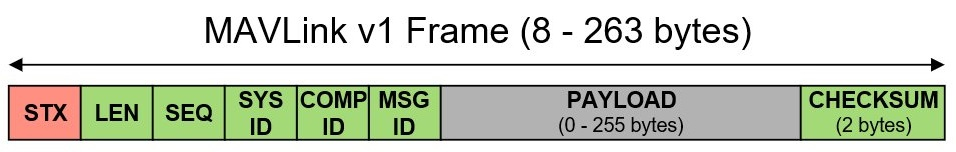
\includegraphics[width=0.8\textwidth]{images/packet_mavlink_v1.jpg}
    \caption{La struttura di un messaggio MAVLink 1.0}
\end{figure}

Per quanto riguarda la dimensione dei pacchetti MAVLink 1.0:

\begin{itemize}
    \item La dimensione \textbf{minima} di un pacchetto MAVLink 1.0 è di 8 bytes (quando \textbf{non} è presente un payload, tipicamente quando si ha a che fare con dei pacchetti di ACK);
    \item La dimensione \textbf{massima} di un pacchetto MAVLink 1.0 è di 263 bytes (8 bytes di header + 255 bytes di payload, quando quest'ultimo è completamente "riempito").
\end{itemize}

\newpage

\subsubsection{MAVLink 2.0: struttura di un pacchetto}

Con il rilascio della versione 2.0 delle specifiche del protocollo, la struttura di un pacchetto è variata leggermente.

In particolare:

\begin{itemize}
    \item Sono stati aggiunti due nuovi membri dell'header: \texttt{CMPFLAGS} e \texttt{INCFLAGS};
    \item È stato aggiunto il supporto alla \textbf{firma digitale del pacchetto};\\
\end{itemize}
Un frame MAVLink 2.0 è quindi strutturato come segue:

\begin{itemize}
    \item Start of Text (\texttt{STX}, chiamato anche \texttt{MAGIC}): un byte che rappresenta l'inizio di un frame MAVLink. Nella versione 2.0 del protocollo questo byte assume un valore fisso: \texttt{0xFD};
    \item Payload Length (\texttt{LEN}): un byte che rappresenta la \textbf{lunghezza in byte} del payload. Poiché questo campo è formato da un solo byte, la lunghezza del payload \textbf{non può superare i 255 bytes};
    \item Incompatibility Flags (\texttt{INCFLAGS}): un byte che rappresenta quelle features del protocollo che \textbf{devono essere tassativamente supportate} da chi riceve il pacchetto poiché \textbf{ne alterano la struttura}. In caso contrario, le specifiche del protcollo indicano che il pacchetto deve essere \textbf{scartato}. L'unico valore attualmente supportato è \texttt{0x01}, che rappresenta la possibilità di \textbf{firmare il messaggio};
    \item Compatibility Flags (\texttt{CMPFLAGS}): un byte che indica la presenza di features "aggiuntive" che, anche se non supportate dal ricevente \textbf{non pregiudicano} la deserializzazione del pacchetto e che quindi lo scarto delpacchetto non è per forza necessario. Un esempio è una flag che denota un pacchetto "ad alta priorità".
    \item Packet Sequence Number (\texttt{SEQ}): un byte che rappresenta il numero di sequenza del pacchetto nel contesto di una comunicazione. Serve principalmente per la \textbf{detection} di \textbf{perdita} dei pacchetti e degli errori in generale;
    \item System ID (\texttt{SYSID}): un byte che rappresenta l'ID del \textbf{mittente} del messaggio. Non è possibile indicare 0 (l'indirizzo di broadcast) come mittente poiché viene interpretato come non valido dal parser;
    \item Component ID (\texttt{COMPID}): un byte che rappresenta la \textbf{componente} del veicolo che ha generato il messaggio (una videocamera o un qualche accessorio);
    \item Message ID (\texttt{MSGID}): \textbf{tre bytes} che rappresentano il \textbf{Message ID} del contenuto del payload. Serve alla libreria per identificare il messaggio eselezionare il parser più adatto per interpretare il contenuto e deserializzarlo. Con l'aumento della dimensione di questo campo è possibile supportare un numero più grande di messaggi e di rendere la libreria ancora più flessibile rispetto a prima;
    \item Payload (\texttt{PAYLOAD}): un vettore di byte di \textbf{al più} 255 bytes (si veda il ragionamento fatto in precedenza) che contiene i dati veri e propri scambiati tra l'UAV e la GCS;
    \item CRC (+ CRC Extra) (\texttt{CHECKSUM}): due bytes: \begin{itemize}
        \item Il primo rappresenta il checksum del messaggio (nel suo calcolo non viene considerato \texttt{STX});
        \item Il secondo (denominato \texttt{CRC\_EXTRA}) rappresenta il CRC della \textbf{struttura della definizione XML del messaggio}. Ciò permette alle due parti della comunicazione di assicurarsi di star considerando messaggi definiti allo stesso modo.
    \end{itemize}
\end{itemize}

Oltre all'header ed al payload, il protocollo MAVLink 2.0 introduce anche la possibilità di aggiungere (\textit{append}) una \textbf{firma digitale} ad un frame. Tale campo è lungo esattamente \textbf{13 bytes}.

\newpage

Di seguito è presente un riepilogo della struttura di un pacchetto MAVLink nella sua revisione 2.0:

\begin{figure}[H]
    \centering
    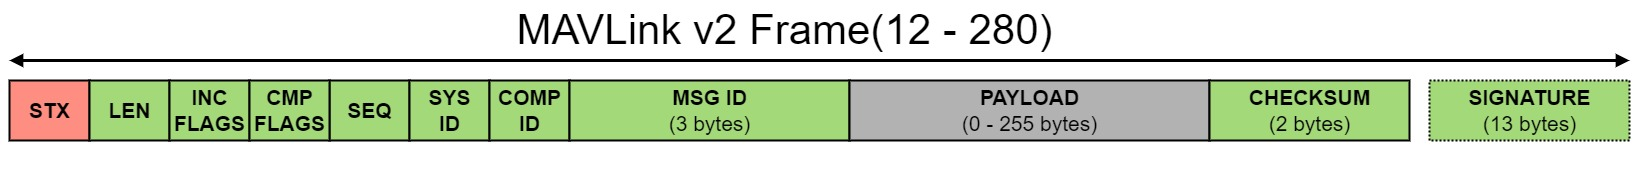
\includegraphics[width=0.8\textwidth]{images/packet_mavlink_v2.jpg}
    \caption{La struttura di un messaggio MAVLink 2.0}
\end{figure}

Alla luce di tutte le informazioni qui sopra riportate, riguardo la dimensione di un frame MAVLink 2.0 è possibile menzionare che:

\begin{itemize}
    \item La dimensione \textbf{minima} di un pacchetto MAVLink 2.0 (senza payload e senza firma) è di \textbf{12 bytes};
    \item La dimensione \textbf{massima} di un pacchetto MAVLink 2.0 (con payload "riempito" e con apposta una firma digitale) è di \textbf{280 bytes} (\textbf{12} bytes di header + \textbf{255} bytes di payload + \textbf{13} bytes di firma). 
\end{itemize}

\subsubsection{Scelta del protocollo}
Poiché l'uso del protocollo MAVLink 1.0 è ancora ampiamente diffuso, è stato necessario implementare un meccanismo di "definizione" della versione del protocollo da utilizzare per una comunicazione: una sorta di \textbf{handshaking} preliminare la cui struttura viene riportata di seguito:

\begin{itemize}
    \item La \textbf{Ground Control Station} invia il messaggio \texttt{MAV\_CMD\_REQUEST\_PROTOCOL\_VERSION} al drone, richiedendo quindi la versione del protocollo in uso dal veicolo ed iniziando contemporaneamente un \textit{countdown di timeout};
    \item L'UAV a questo punto può rispondere in due modi: \begin{itemize}
        \item Se è presente il supporto per il protocollo MAVLink 2.0, risponderà con il messaggio di ACK \texttt{PROTOCOL\_VERSION} formattato come frame MAVLink 2.0;
        \item Se invece non vi è supporto per MAVLink 2.0, risponderà con un \textbf{NACK} e, in caso di assenza di procedure apposite, \textbf{scarterà il messaggio precedente} e non risponderà affatto.
    \end{itemize}
    \item \begin{itemize}
        \item Se la GCS riceve il messaggio \texttt{PROTOCOL\_VERSION} allorà verrà effettuato lo \textit{switch} alla versione 2.0 del protocollo.
        \item Se viene ricevuto un NACK oppure si giunge al timeout, viene utilizzata la versione 1.0 del protocollo poiché evidentemente l'UAV non è riuscito ad interpretare in maniera corretta il frame precedente.
        \end{itemize} 
\end{itemize}

Di seguito è presente una rappresntazione grafica dell'handshaking appena descritto.

\begin{figure}[H]
    \centering
    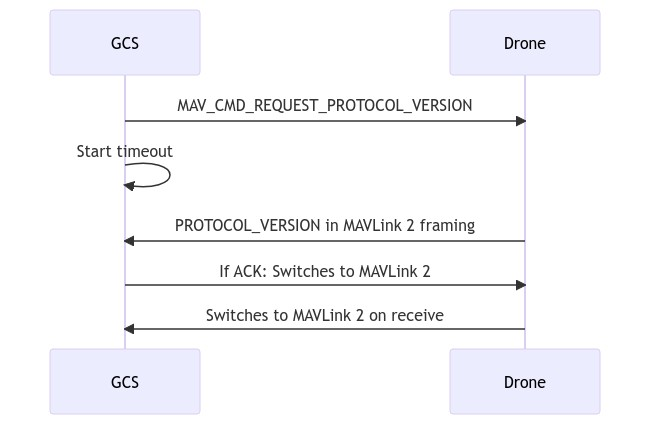
\includegraphics[width=0.8\textwidth]{images/handshake_mavlink.jpeg}
    \caption{L'handshake effettuato per stabilire la versione del protocollo da utilizzare}
\end{figure}

\newpage
\printbibliography[title={Riferimenti bibliografici e risorse consultate}]
\end{document}